\chapter{Introduction}

As the boundaries of the definition of robotics are expanding multi-robot systems are increasingly finding its application in various fields. In many applications, including robots in a cluttered environment like a retail store or search and rescue operation and extremely uncertain environment like planetary exploration or surveillance, one of the key challenges is to map the environment and localize the robot simultaneously. This problem is called Simultaneous Localization and Mapping (SLAM) which deals with fusing different sensor measurements to develop a consistent picture of the environment. With the solutions to \textit{single robot} SLAM getting more matured than ever coupled with the rise of self-driving cars the path forward is to develop solutions for a team of robot explorers which split up at a pathway fork and later meet again to share and merge their maps. Also, with multiple robots, the environment could be mapped more robustly and significantly faster. In particular, we deal with developing a \textit{centralized} optimal map by fusing the measurement estimates from all the robots. Combining the measurements and estimates from multiple robots for centralized mapping is important because it helps to avoid the data redundancy in the overlapping areas and allow the robots to \textit{help each other out} in case of localization loss. Multi-robot SLAM has been extensively studied since the last decade leading to the development of several algorithms \cite{howardmulti,thrunmulti,zhoumulti}. The multi-robot scenario also introduces several key issues on top of a single robot case. A large body of the previous work try to address these issues (listed below) in different ways, 

\begin{enumerate}
\item Globally consistent robot pose initialization.
\item Direct and indirect encounters.
\item Multi-robot data association
\end{enumerate} 

\paragraph{}
For multi-robot SLAM, we use \textit{factor graphs} \cite{factorgraph} as the underlying framework for state estimation. This work proposes a method to quickly and efficiently fuse the factor graphs of the encountering robots and also address the aforementioned issues simultaneously.

\begin{figure}
\centering
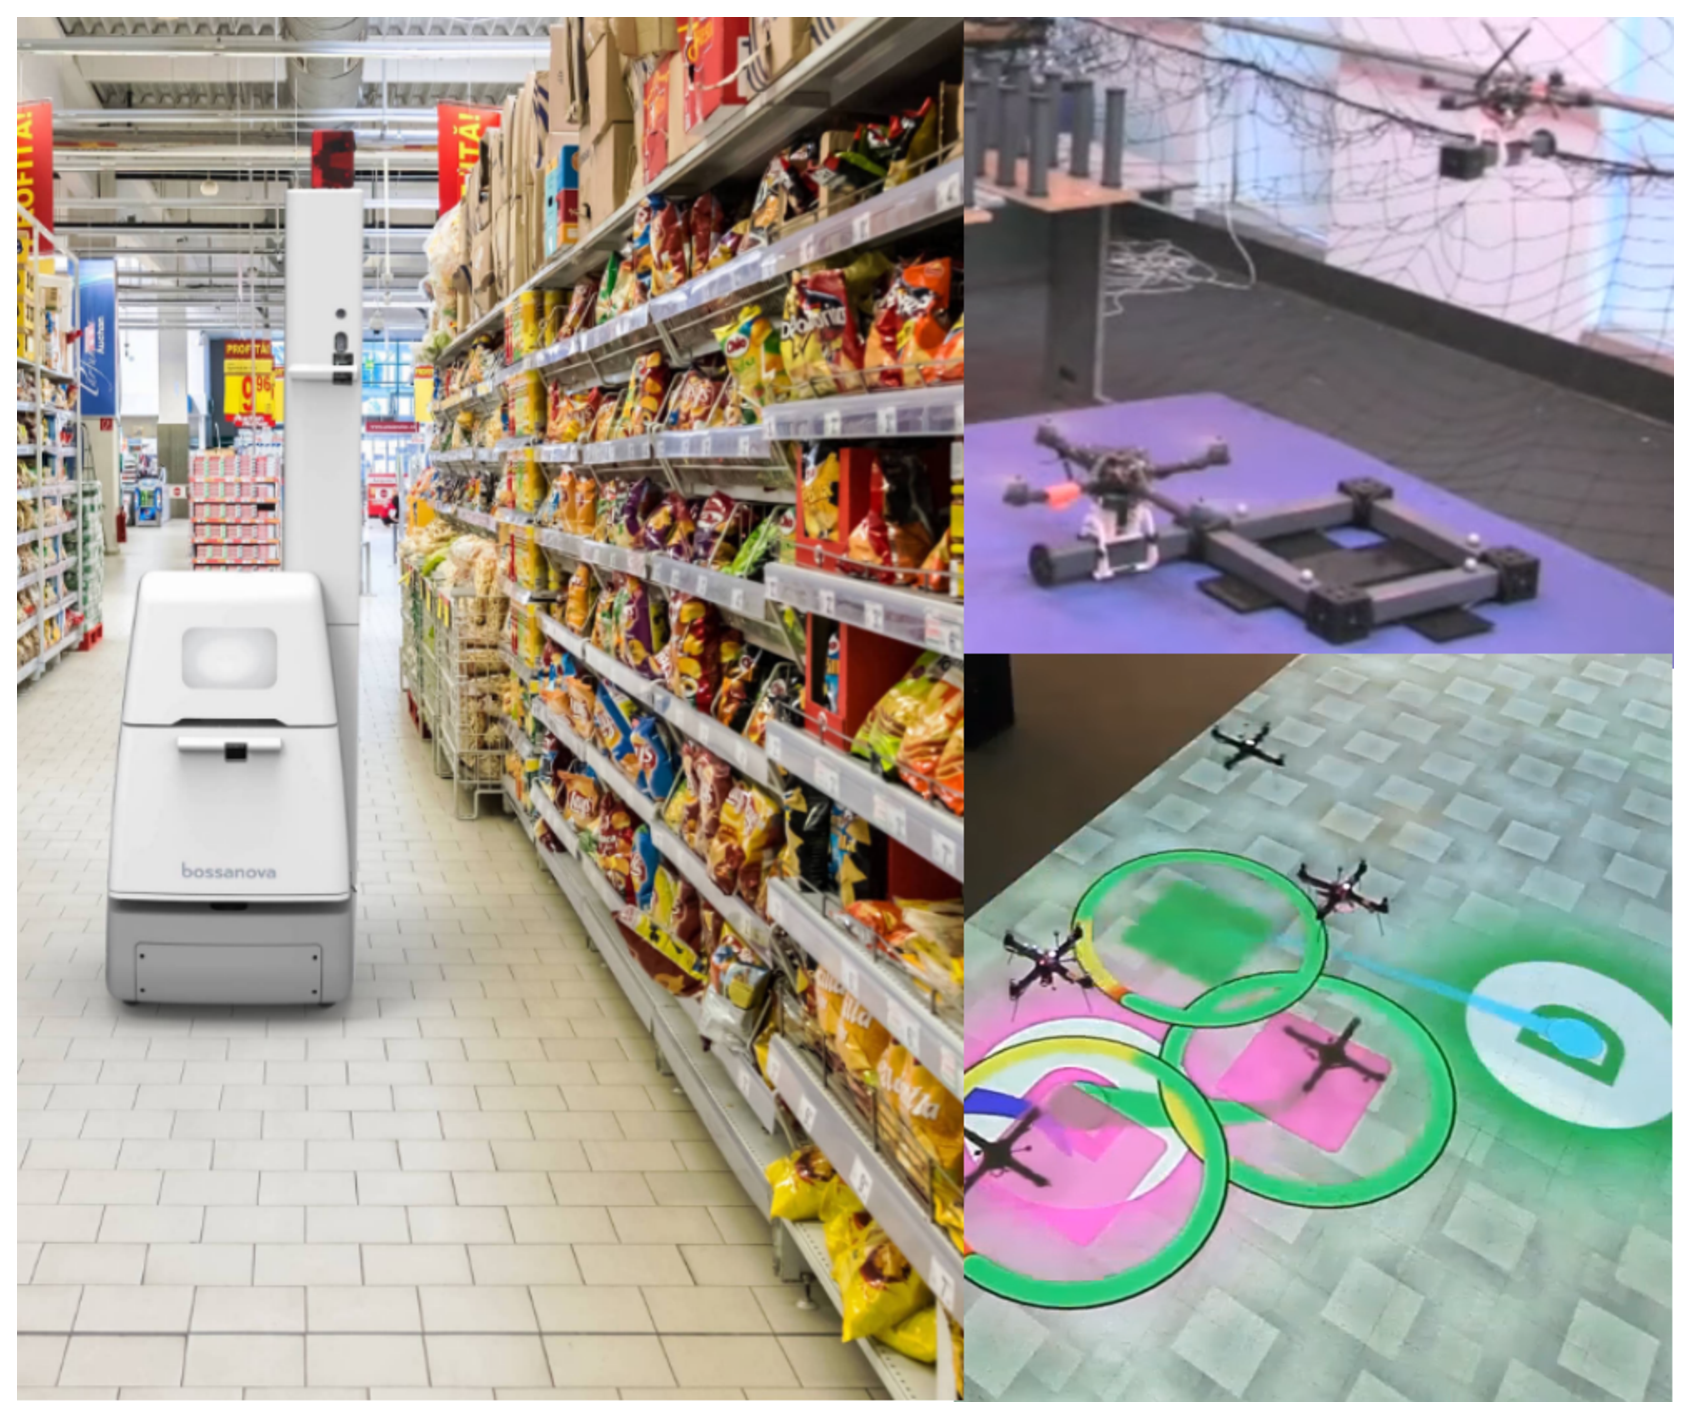
\includegraphics[width=\textwidth]{Chapters/figures1/swarm_safe.eps}
\label{fig:intro}
\caption{Clockwise from left: 1) A mobile robot navigating in a retail store to provide inventory solutions. They are designed to collaborate with other robots at the end of scanning an aisle. 2) Swarm of robots teaming up in a cooperative task of building lego blocks at Grasp Laboratory, University of Pennsylvania. 3) Decentralized control and planning of a multi-robot system at University of New Hampshire.}
\end{figure}

\section{Thesis}

My thesis in this dissertation is the following:

\begin{center}
\textit{Ordering the variables of the fused factor graph using the ordering of the parent factor graphs provides a superior alternative to the complete reordering approach that is fast, efficient and also numerically stable. Also, by introducing the concept of ``global nail" the issue of relative pose graph initialization for different robots is solved.}
\end{center}

\paragraph{}
I split this thesis into three claims that correspond to the Chapters \ref{chap:three}, \ref{chap:four} and  \ref{chap:five} respectively. The goal of my research is efficient factor graph fusion, globally consistent pose initialization for all the robots and rapid multi-channel object detection as explained below:

\begin{enumerate}
\item \textit{Fused Graph Ordering:} Variable reordering is a technique used to retain the sparsity of the factor graph during its factorization. This chapter proposes a numerically stable variable ordering strategy for the fused graph by reusing the parent graph ordering that is faster than the naive approach of complete reordering (Chapter \ref{chap:three}). 

\item \textit{Multi-robot Pose Graph Initialization:} Factor Graph is also referred as Pose Graph in the SLAM context. This chapter introduces a new type of error function used as a factor in the factor graph to estimate the globally consistent trajectory for the robots starting at unknown relative initial positions.

\item \textit{Multi-robot Data Association:} This is another common problem in multi-robot mapping that deals with unknown robot identity during a robot-robot encounter. The experimental real world dataset has colored fiducials attached to the robots and the environment. An improved version of Viola-Jones rapid detection \cite{violajones} for identifying the fiducials is developed and the computational complexity is studied (Chapter \ref{chap:five}). 
\end{enumerate}

\paragraph{}
In the reminder of this chapter, I lay down the reasoning leading to my thesis.

\section{Efficient Factor Graph Fusion}
In order to be useful for a multi-robot system, SLAM needs to perform at real-time. Offline or batch solutions to SLAM means the robot has to wait until the calculation for the update is finished. Even in the case of multiple robots with a centralized mapping capability, quicker update times are always useful. With the centralized system calculating the best estimate based on measurements received from all the robots, an update sent back to the individual robots could be used to correct or improve the local estimates. 

\paragraph{}
A real-time algorithm should also be able to update the system incrementally. This means that the centralized system should just require the new set of measurements from the individual robots taken after the last time they communicated to make an update. SLAM by nature itself is a sparse problem with the measurements connected temporally almost always. The centralized system should also be able to calculate an update by just using a local portion of the graph being impacted by the new measurements. For example, the measurements from a robot moving down a particular aisle in a retail store are completely independent of the measurements and observations made in a different and far away aisle. So a centralized system recalculating the estimates of the unaffected portions of the map is not a wise option. This incremental requirement for SLAM problem is well studied, particularly by Kaess and Dellart in \cite{kaessisam} and \cite{kaessisam2}. By using the formulation presented in their work and reusing the variable ordering of the graph being combined we come up with an efficient graph fusion strategy (Chapter 3). 

\section{Multi-robot Pose Graph Initialization}
The measurements from multiple robots must be globally consistent to build a unified map of the environment. In order to do this, all the robots should have a prior knowledge about their relative initial positions. It is not necessary or a fair assumption to consider that all the robots of a multi-robot system start at the same position on the map. Any arbitrary value to the initial position will lead to a conflict during a robot-robot encounter in terms of global map alignment. For example, in the case of multiple robots navigating in a large retail store across distinct aisles, lack of knowledge about each robot's initial position gives the freedom to all the independent trajectories to align together in several possible ways. Although there is a closed form solution to resolve the alignment issue with a single robot-robot encounter \cite{zhoumulti} the devised algorithm should be able to continuously and incrementally integrate the incoming measurements to refine the alignment error. 

\paragraph{}
The encounter could also be \textit{indirect} in which multiple robots visit the same portion of the environment at different time instants. In this case, the variable representing the pose of the landmark (or common portion of visit among different robots) is also involved in alignment estimation. It is therefore essential for the algorithm to incorporate indirect encounters in the alignment of the map. In other words, aligning the map is same as finding the globally consistent initial pose for all the robots. A cost function that tries to minimize the alignment error and also supports multiple encounters between the robots is formulated and optimized in Chapter 4.

\section{Multi-robot Data Association}
Data Association, in general, is an important component of SLAM. It is the process of recognizing previously visited landmarks in the environment to refine the map and the robot's path. There are several ways of extracting the features of interest (landmarks) from the environment, ranging from wireless network-based to computer vision techniques. With multiple robots in place the identity of the fellow robots should also be identified on top of the landmarks in the environment. The data association engine should be able to recognize both the landmarks in the environment and the robot IDs from the extracted features. Simultaneously, these type of sophisticated measurements should not consume a large amount of time as it introduces the problem of synchronization and scheduling.

\paragraph{}
In this thesis, an object detection based data association is used to demonstrate the results with the experimental dataset. Although this is not the main concentration of the thesis, an improved Viola-Jones rapid object detection \cite{violajones} is devised to work in the multi-channel image space. As it is able to use multiple image channels beyond color (like depth and intensity), detection could be performed at a much lower resolution saving time per scan. Chapter \ref{chap:five} presents a theoretical study of the time complexity of the improved algorithm.

\section{Organization}
The remainder of the dissertation is organized as follows: The background and related work is discussed separately for factor graph ordering and multi-robot map alignment in Chapter 3 and Chapter 4 respectively. The next chapter formally introduces the factor graph and the Bayes tree data structure often used throughout my work. In Chapter \ref{chap:two}, a set of key terminologies from graph theory and sparse linear algebra literature are also explained for the sake of better understanding and completeness. The novel algorithm to quickly find the variable ordering of the fused graph is presented in Chapter 3. Experimental results on the standard real world datasets from the sparse linear algebra literature is also presented at the end of Chapter 3. Chapter 4 deals with the problem of pose graph initialization or map alignment and gives a solution by devising an appropriate cost function and ``global nail". A detailed numerical section, sensor models $\&$ software library used and demonstration of experiments is presented in Chapter 5. The conclusions and the potential future work are also discussed in the same chapter. Finally, Chapter \ref{chap:five} presents the improved rapid object detection for multi-channel images.





